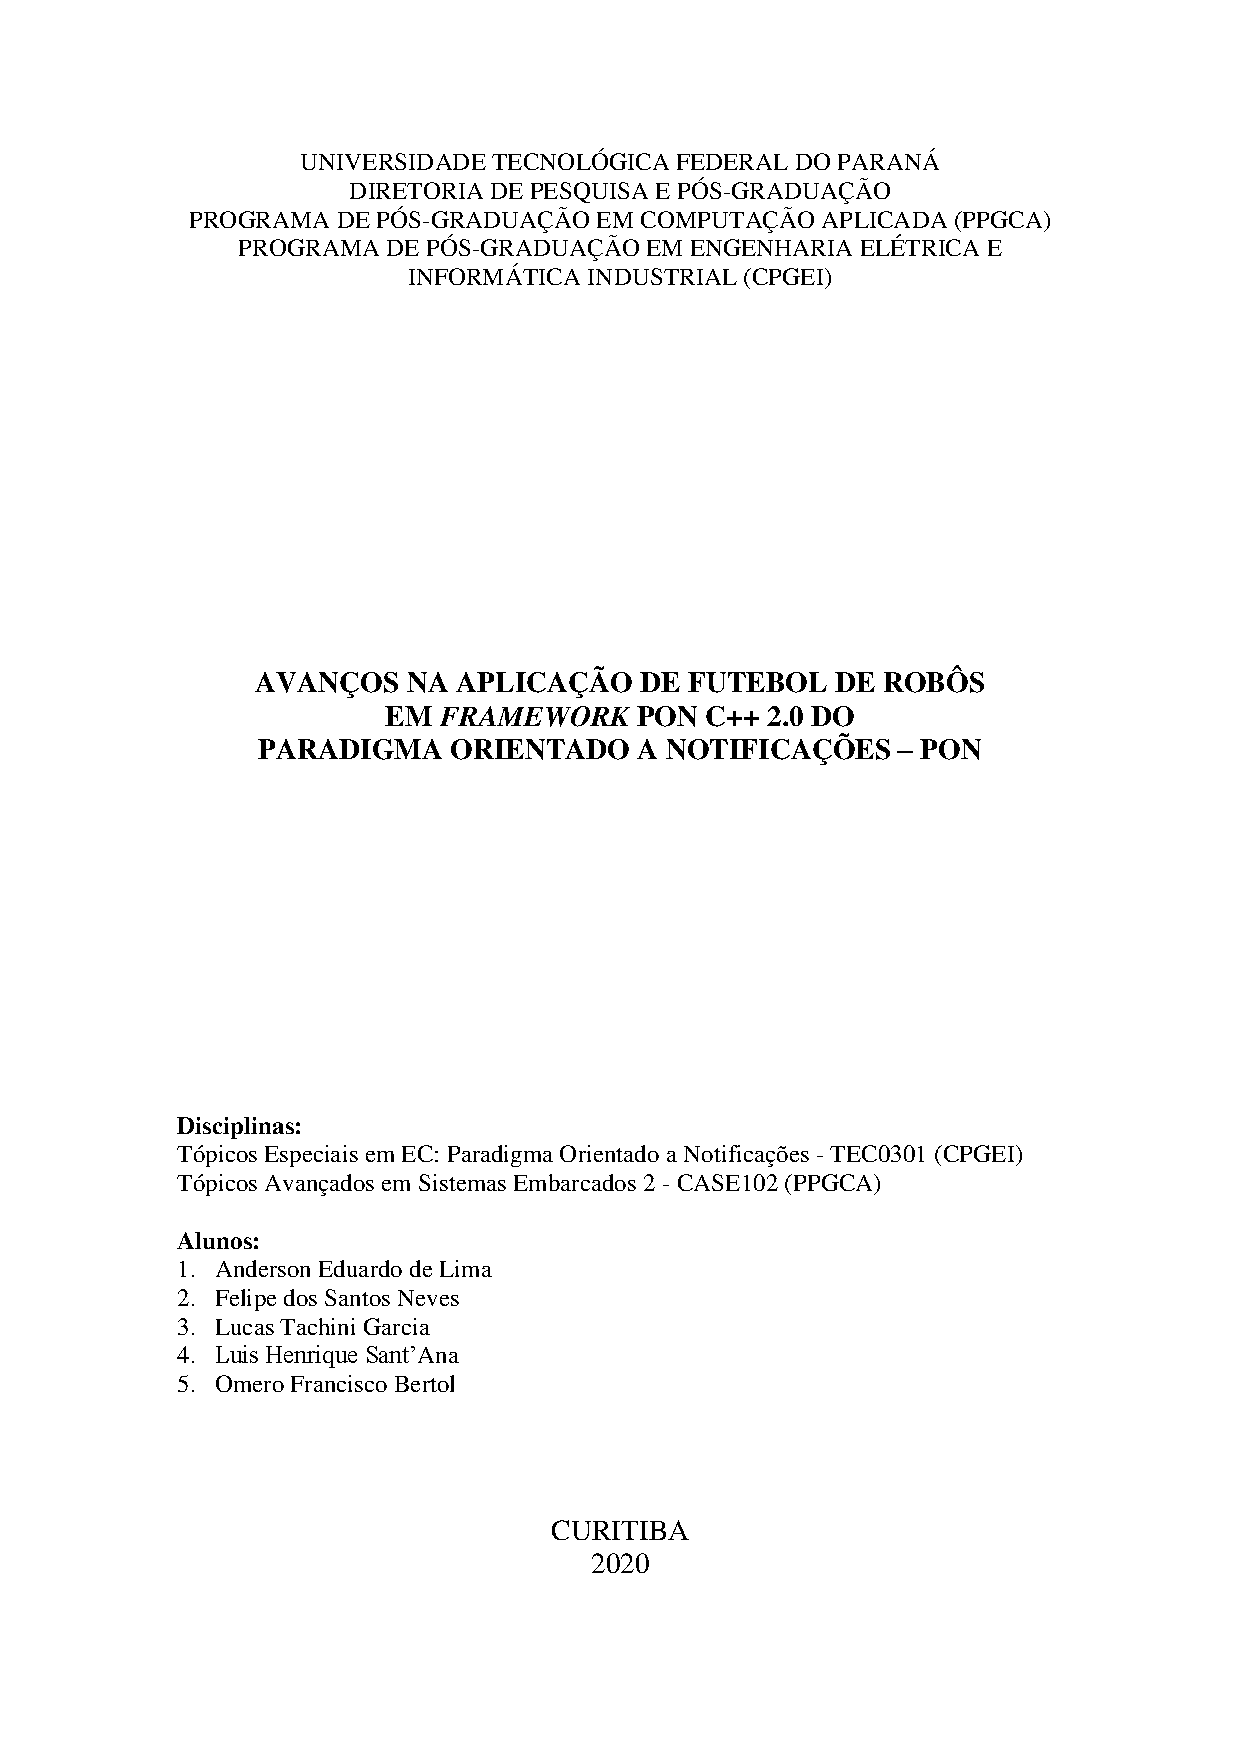
\includepdf[pages={1}, scale=0.8, pagecommand=\chapter*{Apêndice A}\label{ch:apendice_futebol}]{../extra/futebol_robos.pdf}
\includepdf[pages={2-21}, scale=0.8]{../extra/futebol_robos.pdf}

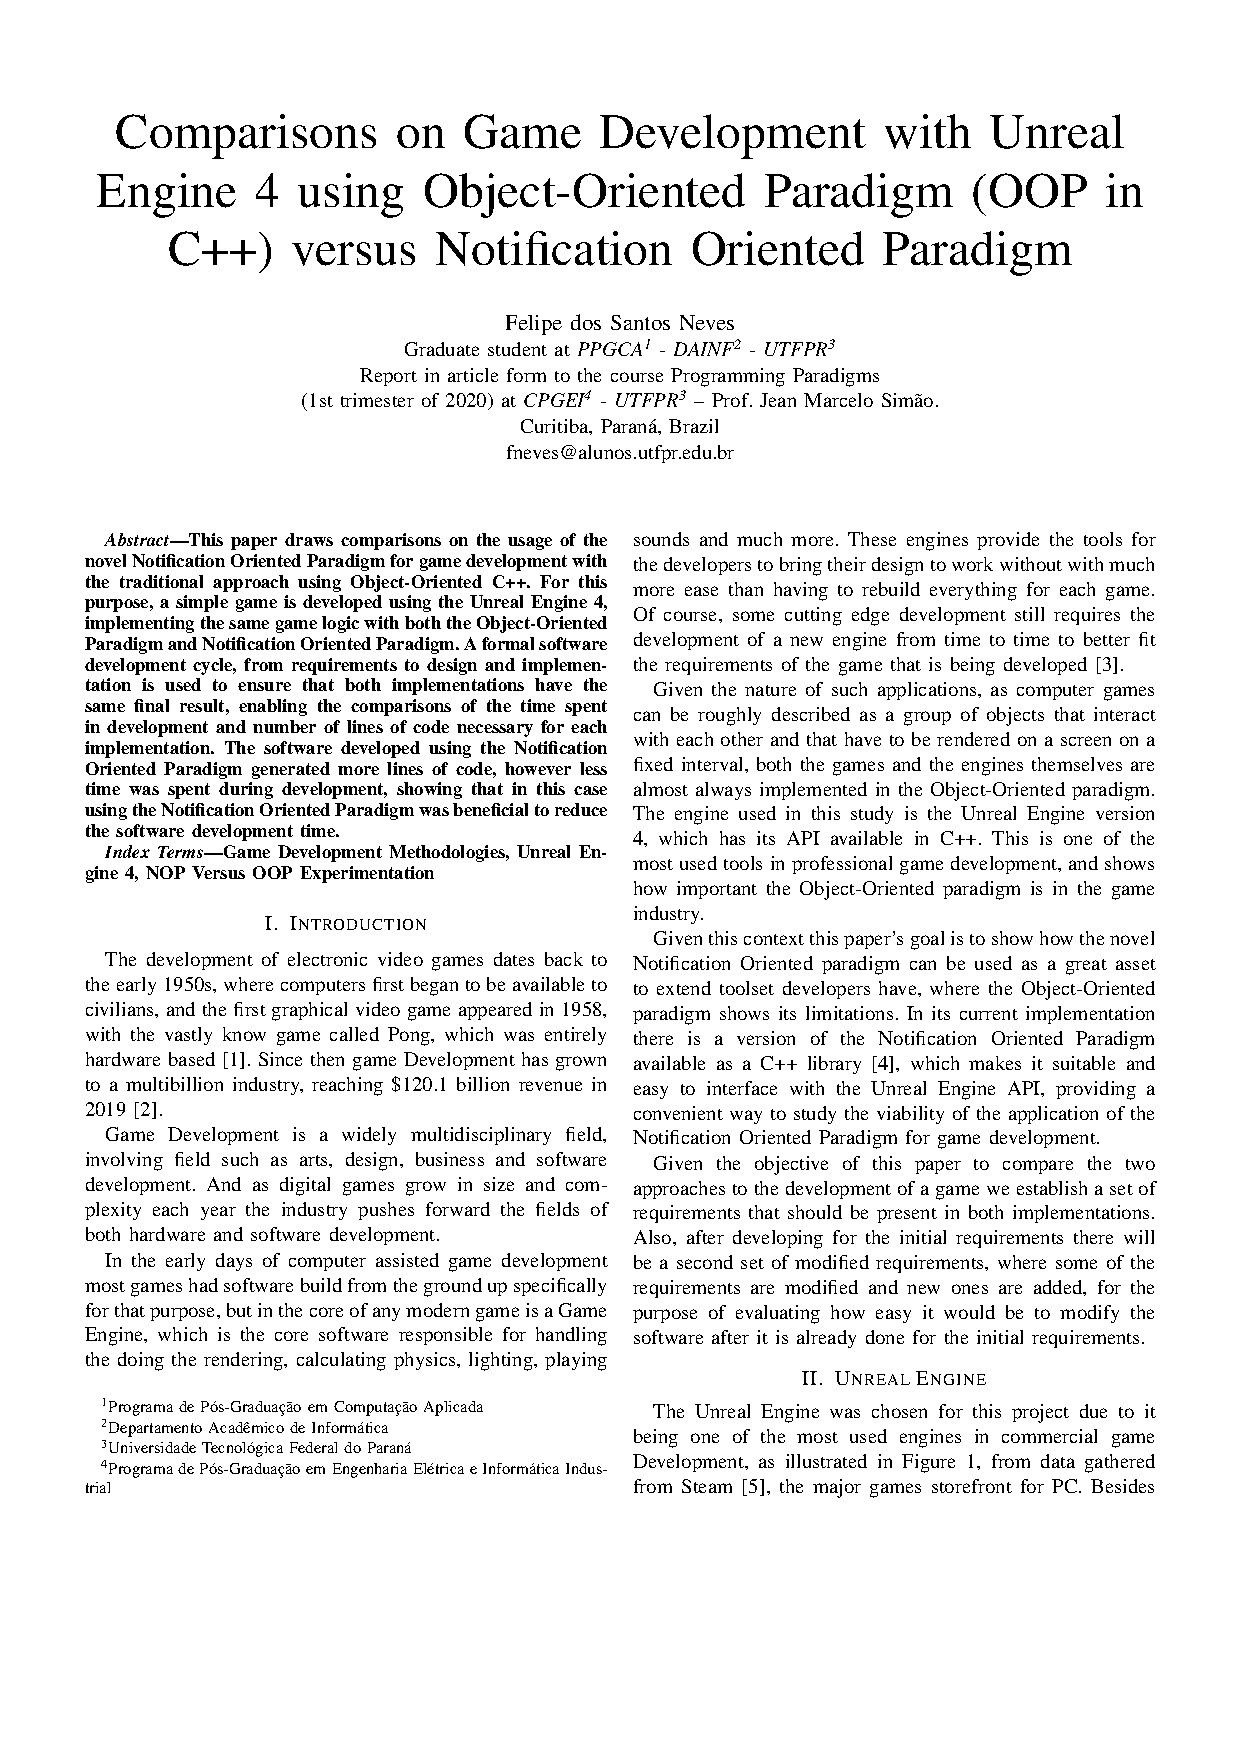
\includepdf[pages={1}, scale=0.8, pagecommand=\chapter*{Apêndice B}\label{ch:apendice_nopunreal}]{../extra/nop_unreal.pdf}
\includepdf[pages={2-10}, scale=0.8]{../extra/nop_unreal.pdf}

%\chapter*{Apêndice D}\label{ch:neves_icist}\smallskip
%%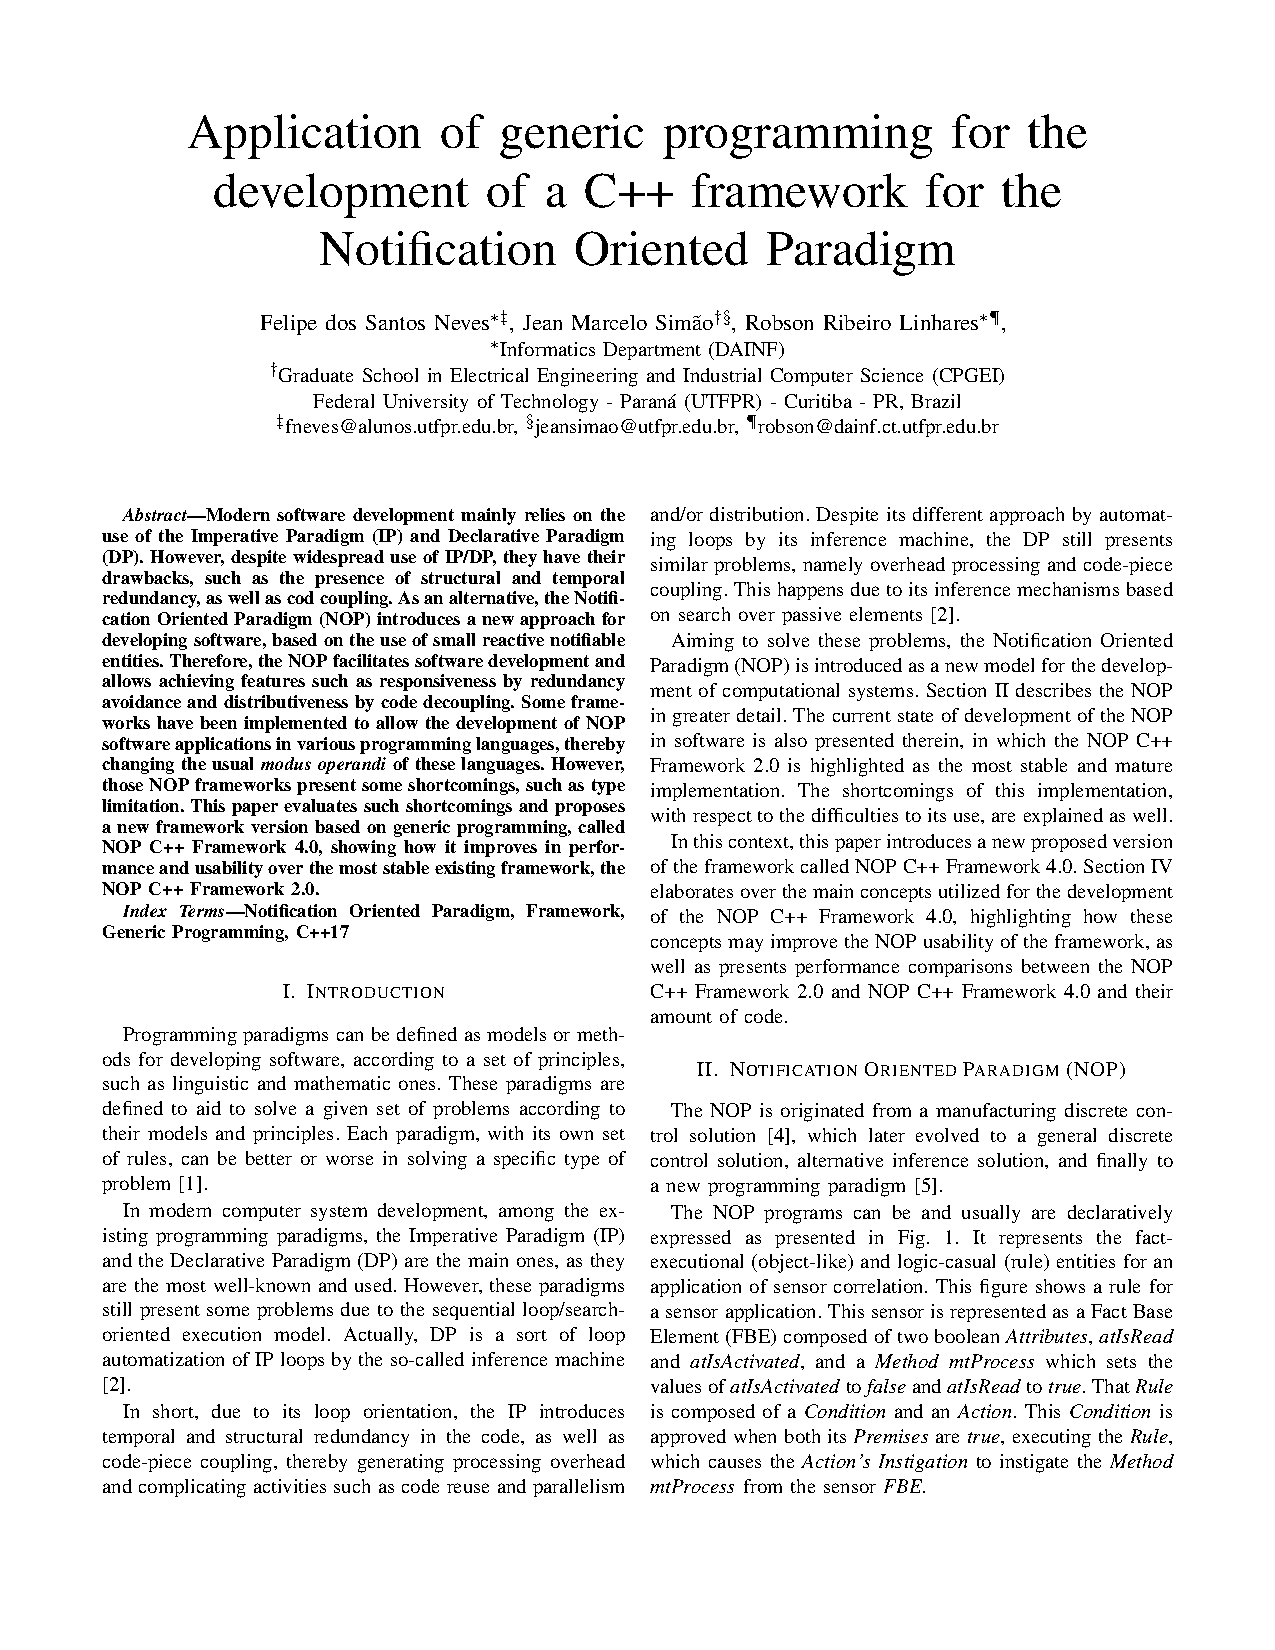
\includepdf[scale=0.85,pages=1]{../extra/icist_neves_290421.pdf}
%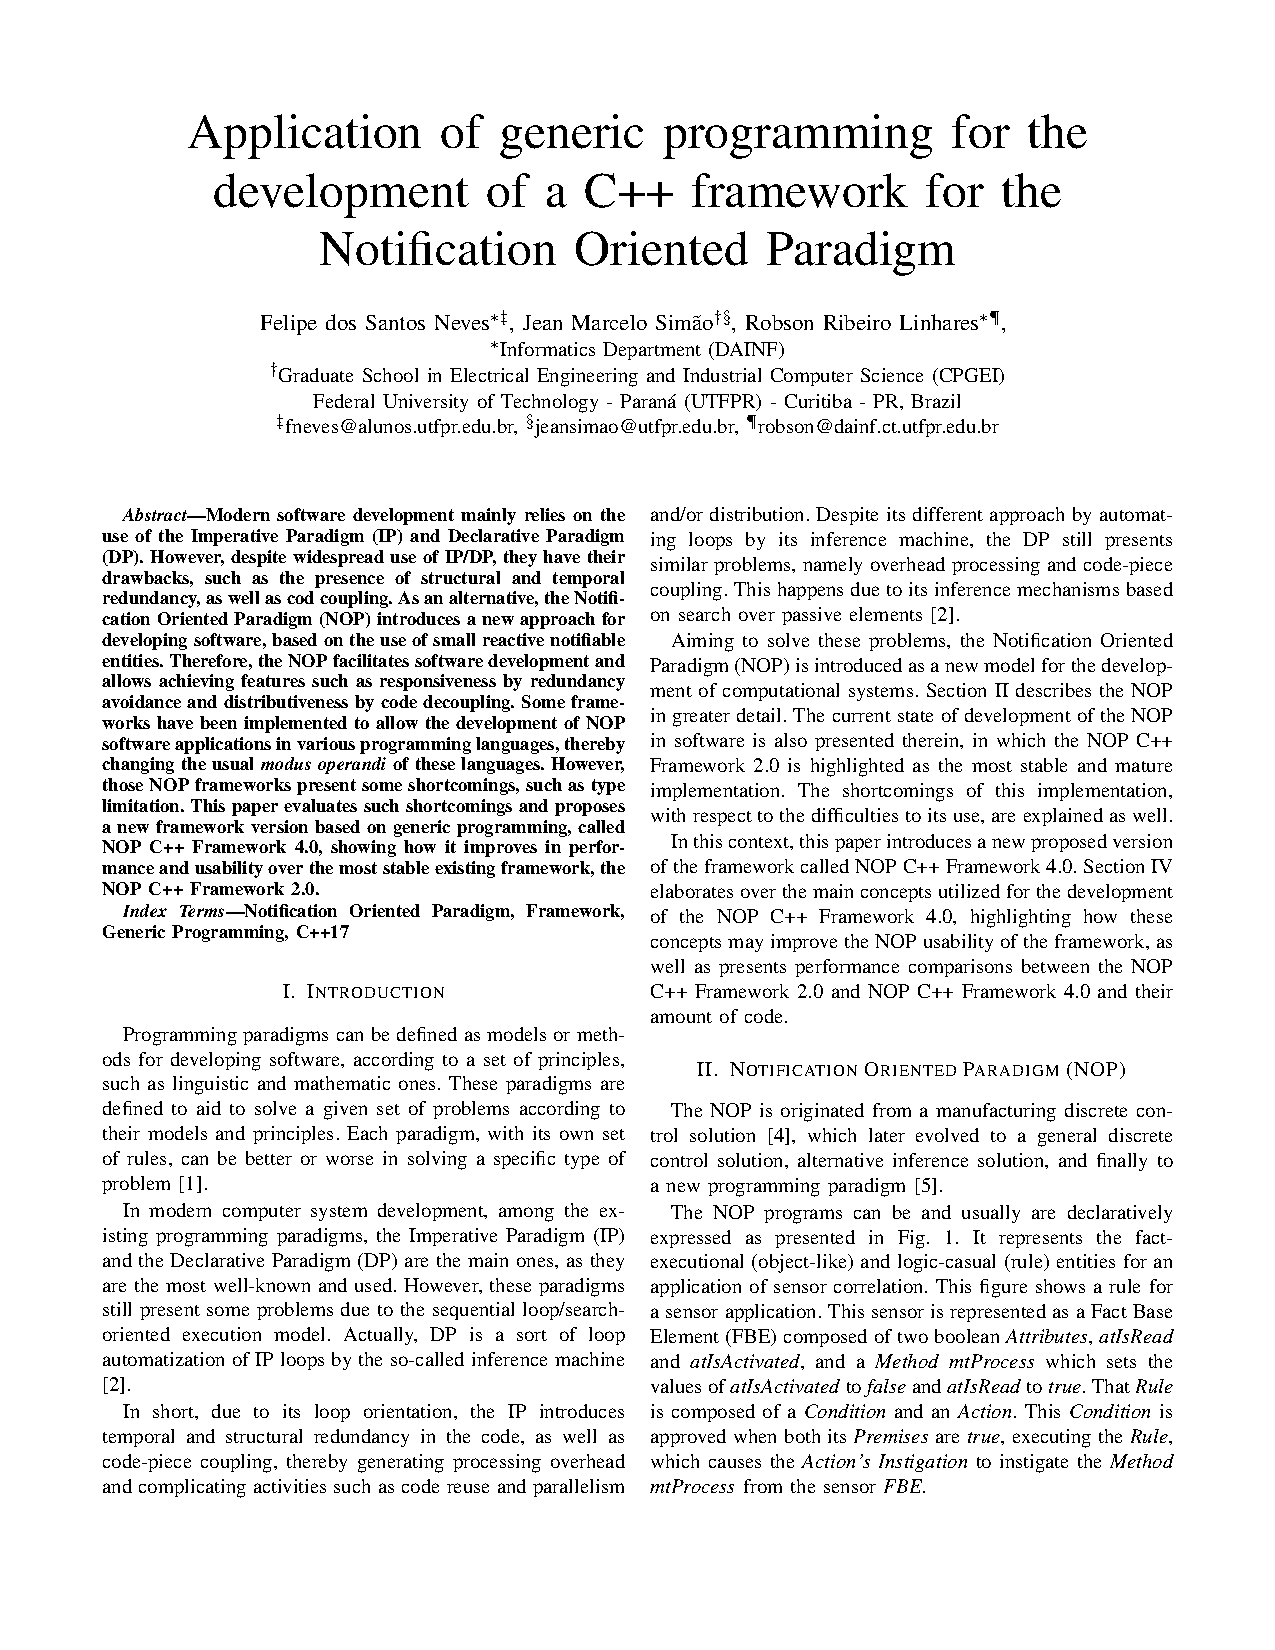
\includepdf[pages={1-6}]{../extra/icist_neves_290421.pdf}

\begin{comment}
\chapter*{Apêndice C}\label{ap:fw_full} 

\section*{Código-fonte do \textit{Framework} PON C++ 4.0}

O código completo do \textit{Framework} PON C++ 4.0 atualizado também pode ser consultado no servidor
de artefatos do PON, uma vez que se tenha acesso a ele (via login e senha) em
\url{https://nop.dainf.ct.utfpr.edu.br/nop-implementations/frameworks/nop-framework-cpp-4}.

\subsection*{License}
\lstinputlisting[language=C++,nolol=true]{../code/framework/LICENSE}
\subsection*{libnop/action.h}
\lstinputlisting[language=C++,nolol=true]{../code/framework/include/libnop/action.h}
\subsection*{libnop/attribute.h}
\lstinputlisting[language=C++,nolol=true]{../code/framework/include/libnop/attribute.h}
\subsection*{libnop/condition.h}
\lstinputlisting[language=C++,nolol=true]{../code/framework/include/libnop/condition.h}
\subsection*{libnop/definitions.h}
\lstinputlisting[language=C++,nolol=true]{../code/framework/include/libnop/definitions.h}
\subsection*{libnop/fbe.h}
\lstinputlisting[language=C++,nolol=true]{../code/framework/include/libnop/fbe.h}
\subsection*{libnop/framework.h}
\lstinputlisting[language=C++,nolol=true]{../code/framework/include/libnop/framework.h}
\subsection*{libnop/instigation.h}
\lstinputlisting[language=C++,nolol=true]{../code/framework/include/libnop/instigation.h}
\subsection*{libnop/logger.h}
\lstinputlisting[language=C++,nolol=true]{../code/framework/include/libnop/logger.h}
\subsection*{libnop/observable.h}
\lstinputlisting[language=C++,nolol=true]{../code/framework/include/libnop/observable.h}
\subsection*{libnop/observer.h}
\lstinputlisting[language=C++,nolol=true]{../code/framework/include/libnop/observer.h}
\subsection*{libnop/premise.h}
\lstinputlisting[language=C++,nolol=true]{../code/framework/include/libnop/premise.h}
\subsection*{libnop/rule.h}
\lstinputlisting[language=C++,nolol=true]{../code/framework/include/libnop/rule.h}
\subsection*{libnop/scheduler.h}
\lstinputlisting[language=C++,nolol=true]{../code/framework/include/libnop/scheduler.h}
\subsection*{action.cpp}
\lstinputlisting[language=C++,nolol=true]{../code/framework/src/action.cpp}
\subsection*{attribute.cpp}
\lstinputlisting[language=C++,nolol=true]{../code/framework/src/attribute.cpp}
\subsection*{condition.cpp}
\lstinputlisting[language=C++,nolol=true]{../code/framework/src/condition.cpp}
\subsection*{fbe.cpp}
\lstinputlisting[language=C++,nolol=true]{../code/framework/src/fbe.cpp}
\subsection*{instigation.cpp}
\lstinputlisting[language=C++,nolol=true]{../code/framework/src/instigation.cpp}
\subsection*{logger.cpp}
\lstinputlisting[language=C++,nolol=true]{../code/framework/src/logger.cpp}
\subsection*{observable.cpp}
\lstinputlisting[language=C++,nolol=true]{../code/framework/src/observable.cpp}
\subsection*{observer.cpp}
\lstinputlisting[language=C++,nolol=true]{../code/framework/src/observer.cpp}
\subsection*{premise.cpp}
\lstinputlisting[language=C++,nolol=true]{../code/framework/src/premise.cpp}
\subsection*{rule.cpp}
\lstinputlisting[language=C++,nolol=true]{../code/framework/src/rule.cpp}
\subsection*{scheduler.cpp}
\lstinputlisting[language=C++,nolol=true]{../code/framework/src/scheduler.cpp}
\end{comment}


\chapter*{Apêndice D}\label{ap:testes}
\subsection*{Conjunto de testes do \textit{Framework} PON C++ 4.0}
\lstinputlisting[language=C++,nolol=true]{../code/framework/libnop_gtest/test.cpp}

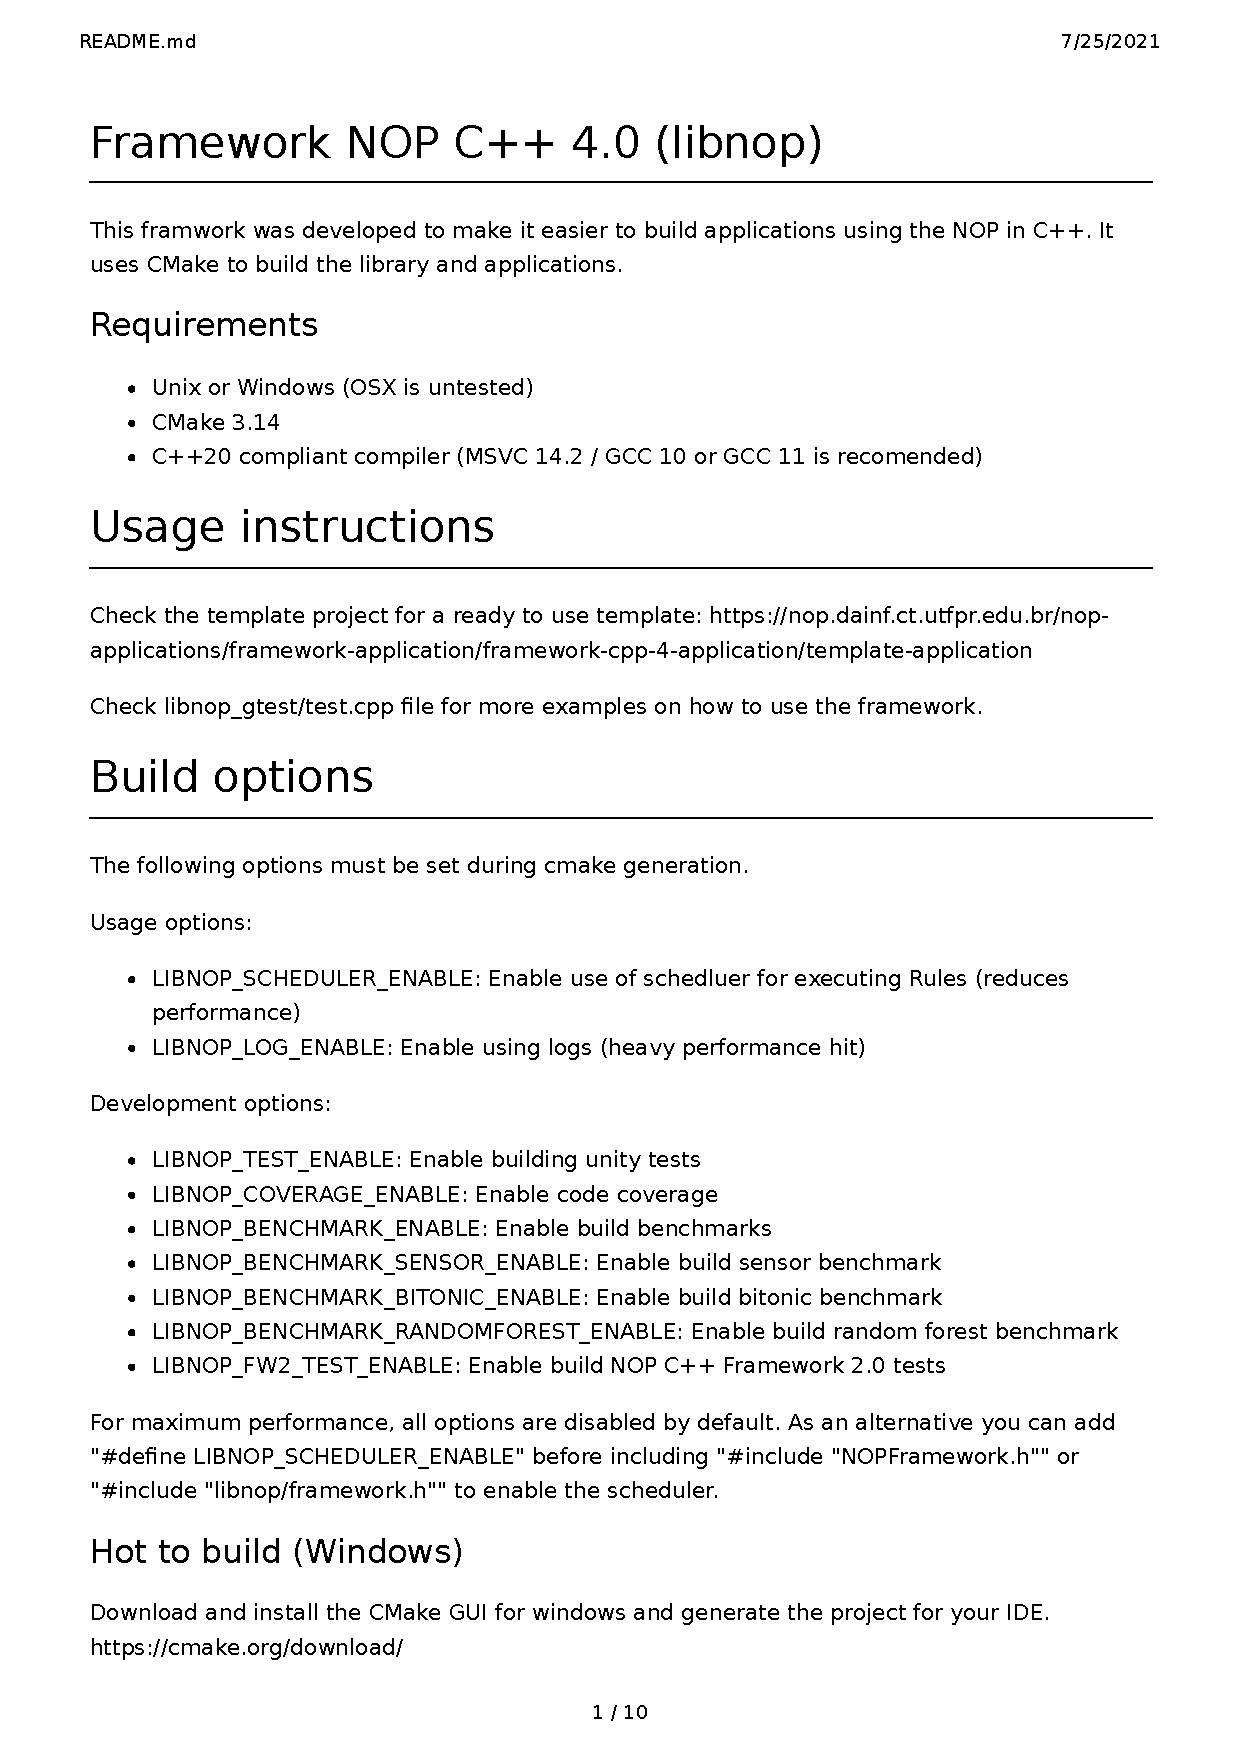
\includepdf[pages={1}, scale=0.7, pagecommand=\chapter*{Apêndice E}\label{ch:manual}]{../extra/README.pdf}
\includepdf[pages={2-10}, scale=0.7]{../extra/README.pdf}

\chapter*{Apêndice F}\label{ap:apendice_mira_alvo}

A aplicação mira ao alvo tem como objetivo ser uma aplicação que realce os
problemas de redundâncias estruturais e temporais, permitindo assim comparações
de desempenho do PON com os demais paradigmas. Neste cenário, ilustrado na
Figura \ref{fig:mira_alvo2}, um conjunto de arqueiros deve atirar em um conjunto
de maçãs, de acordo com o estado das maçãs e da arma de fogo que tem a função de
sinalizar o disparo de início desta interação.

\begin{figure}[!htb]
\centering
\caption{Aplicação mira ao alvo}
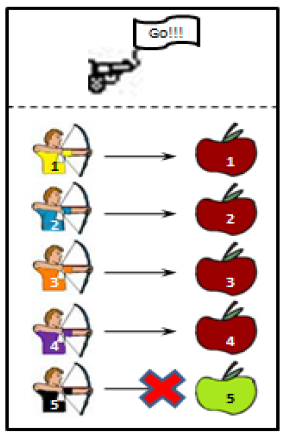
\includegraphics[width=0.45\textwidth]{../figures/mira_alvo_2.PNG}
\smallskip
\fonte{\citeonline{msc_Banaszewski_2009}}
\label{fig:mira_alvo2}
\end{figure}

O Código \ref{cod:mira_alvo} apresenta o desenvolvimento deste cenário com o
\textit{Framework} PON C++ 4.0. A maçã, arqueiro e arma de fogo são
representados, respectivamente, por \textit{NOP4Apple}, \textit{NOP4Archer} e
\textit{NOP4Gun}, enquanto a \textit{Rule} é impplementada em \textit{NOP4GUn}.
  
\begin{lstlisting}[caption = {Código da estrutura do mira ao alvo com o \textit{Framework} PON C++ 4.0},
source = {Autoria própria},
label = {cod:mira_alvo}]
struct NOP4Apple : NOP::FBE {
    NOP::SharedAttribute<std::string> atColor =
        NOP::BuildAttribute<std::string>("GREEN");
    NOP::SharedAttribute<bool> atStatus = NOP::BuildAttribute(true);
    NOP::SharedAttribute<bool> atIsCrossed = NOP::BuildAttribute(false);
};

struct NOP4Archer : NOP::FBE {
    NOP::SharedAttribute<bool> atStatus = NOP::BuildAttribute(true);
};

struct NOP4Gun : NOP::FBE {
    NOP::SharedAttribute<bool> atStatus = NOP::BuildAttribute(false);
};


struct NOP4ArcherRule {
    NOP::SharedRule rule;    
    NOP4ArcherRule(std::shared_ptr<NOP4Apple>& apple,
                    std::shared_ptr<NOP4Archer>& archer,
                    NOP::SharedPremise& prGunIsTrue) {
        rule = NOP::BuildRule(
            NOP::BuildCondition<NOP::Conjunction>(
                NOP::BuildPremise<std::string>(apple->atColor, "RED",
                                                NOP::Equal()),
                NOP::BuildPremise(apple->atStatus, true, NOP::Equal()),
                NOP::BuildPremise(archer->atStatus, true, NOP::Equal()),
                prGunIsTrue),
            NOP::BuildAction(NOP::BuildInstigation(
                [=]() { apple->atIsCrossed->SetValue(true); })));
    }
};
\end{lstlisting}

Durante os experimentos realizados por \citeonline{msc_Banaszewski_2009}, a
aplicação desenvolvida com o \textit{Framework} PON C++ 1.0 apresentou
desempenho um pouco inferior à mesma aplicação desenvolvida com o POO, conforme
apresentado na Figura \ref{fig:mira_alvo_result}. Porém, nos novos testes
realizados com o \textit{Framework} PON C++ 4.0, a aplicação em PON não
conseguiu chegar perto dos mesmos resultados, conforme apresentado na Figura
\ref{fig:mira_alvo_result_2}.

\begin{figure}[!htb]
\centering
\caption{Resultado do experimento mira ao alvo com o \textit{Framework PON C++ 1.0}}
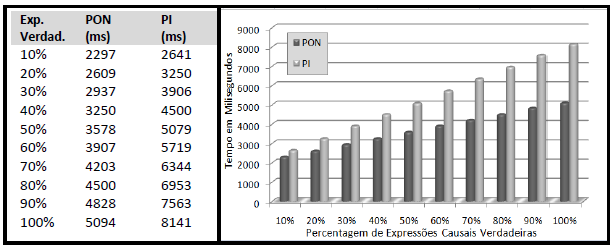
\includegraphics[width=0.9\textwidth]{../figures/mira_alvo_result.PNG}
\smallskip
\fonte{\citeonline{msc_Banaszewski_2009}}
\label{fig:mira_alvo_result}
\end{figure}

A dificuldade em se reproduzir os mesmos resultados pode ser justificada pela
dificuldade em se determinar as condições originais do teste, visto que a versão
do compilador e opções de otimização podem influenciar de forma significa o
desempenho da aplicação. Além disso, processadores com arquiteturas mais
modernas, com os utilizados nos novos testes\footnote{Teste executado em um
computador com processor Ryzen 5 3600 a 3.6GHz e 16 GB de RAM DDR4 a 3000MHz
(dual channel) e sistema operacional Windows 10 64 bits.}, apresentam recursos
que otimizam a execução de operações condicionais e laçoes de repetição, de modo
que são capazes de compensar os efeitos das redundâncias temporais e
estruturais.

\begin{figure}[t!]
\centering
\pgfplotstableread{../data/mira_alvo.data}{\sensorbench}
\begin{tikzpicture}[scale=0.75]
\begin{axis}[width=0.8\linewidth, ylabel=Tempo de execução (ns), %ymode=log,
xlabel=Taxa de aprovação (\%), xmin=0, xmax=100, xmajorticks=true, legend
pos=north west] \addplot [mark=*, red, thick] table [x={rate}, y={poo}]
{\sensorbench}; \addplot [mark=*, blue, thick] table [x={rate}, y={fw4}]
{\sensorbench}; \legend{POO com C++, \textit{Framework} PON C++ 4.0 }
\end{axis}
\end{tikzpicture}
\caption{Resultado do experimento mira ao alvo com o \textit{Framework PON C++ 4.0}}
\fonte{Autoria própria}
\label{fig:mira_alvo_result_2}
\end{figure}


\chapter*{Apêndice G}\label{ap:apendice_bitonic}
\section*{Código-fonte da aplicação Bitonic Sort em PON no \textit{Framework} PON C++ 4.0}
\lstinputlisting[language=C++,nolol=true]{../code/bitonic_sort.cpp}

\chapter*{Apêndice H}\label{ap:bitonic_c}
\section*{Código-fonte da aplicação Bitonic Sort no PP em linguagem de programação C}
\lstinputlisting[language=C++,nolol=true]{../code/bitonic.c}

\chapter*{Apêndice I}\label{ap:rf}
\section*{Código-fonte da aplicação Random Forest em PON no \textit{Framework} PON C++ 4.0}
\lstinputlisting[language=C++,nolol=true]{../code/forest.cpp}
\section*{Código-fonte da aplicação Random Forest em PP na linguagem de programação C}
\lstinputlisting[language=C++,nolol=true]{../code/vivado.c}

\chapter*{Apêndice J}\label{ap:cta}
\section*{Código-fonte da aplicação CTA em LingPON}
\lstinputlisting[language=C++,nolol=true]{../code/cta.nop}
\section*{Código-fonte da aplicação CTA em PON no \textit{Framework} PON C++ 4.0}
\lstinputlisting[language=C++,nolol=true]{../code/cta.cpp}

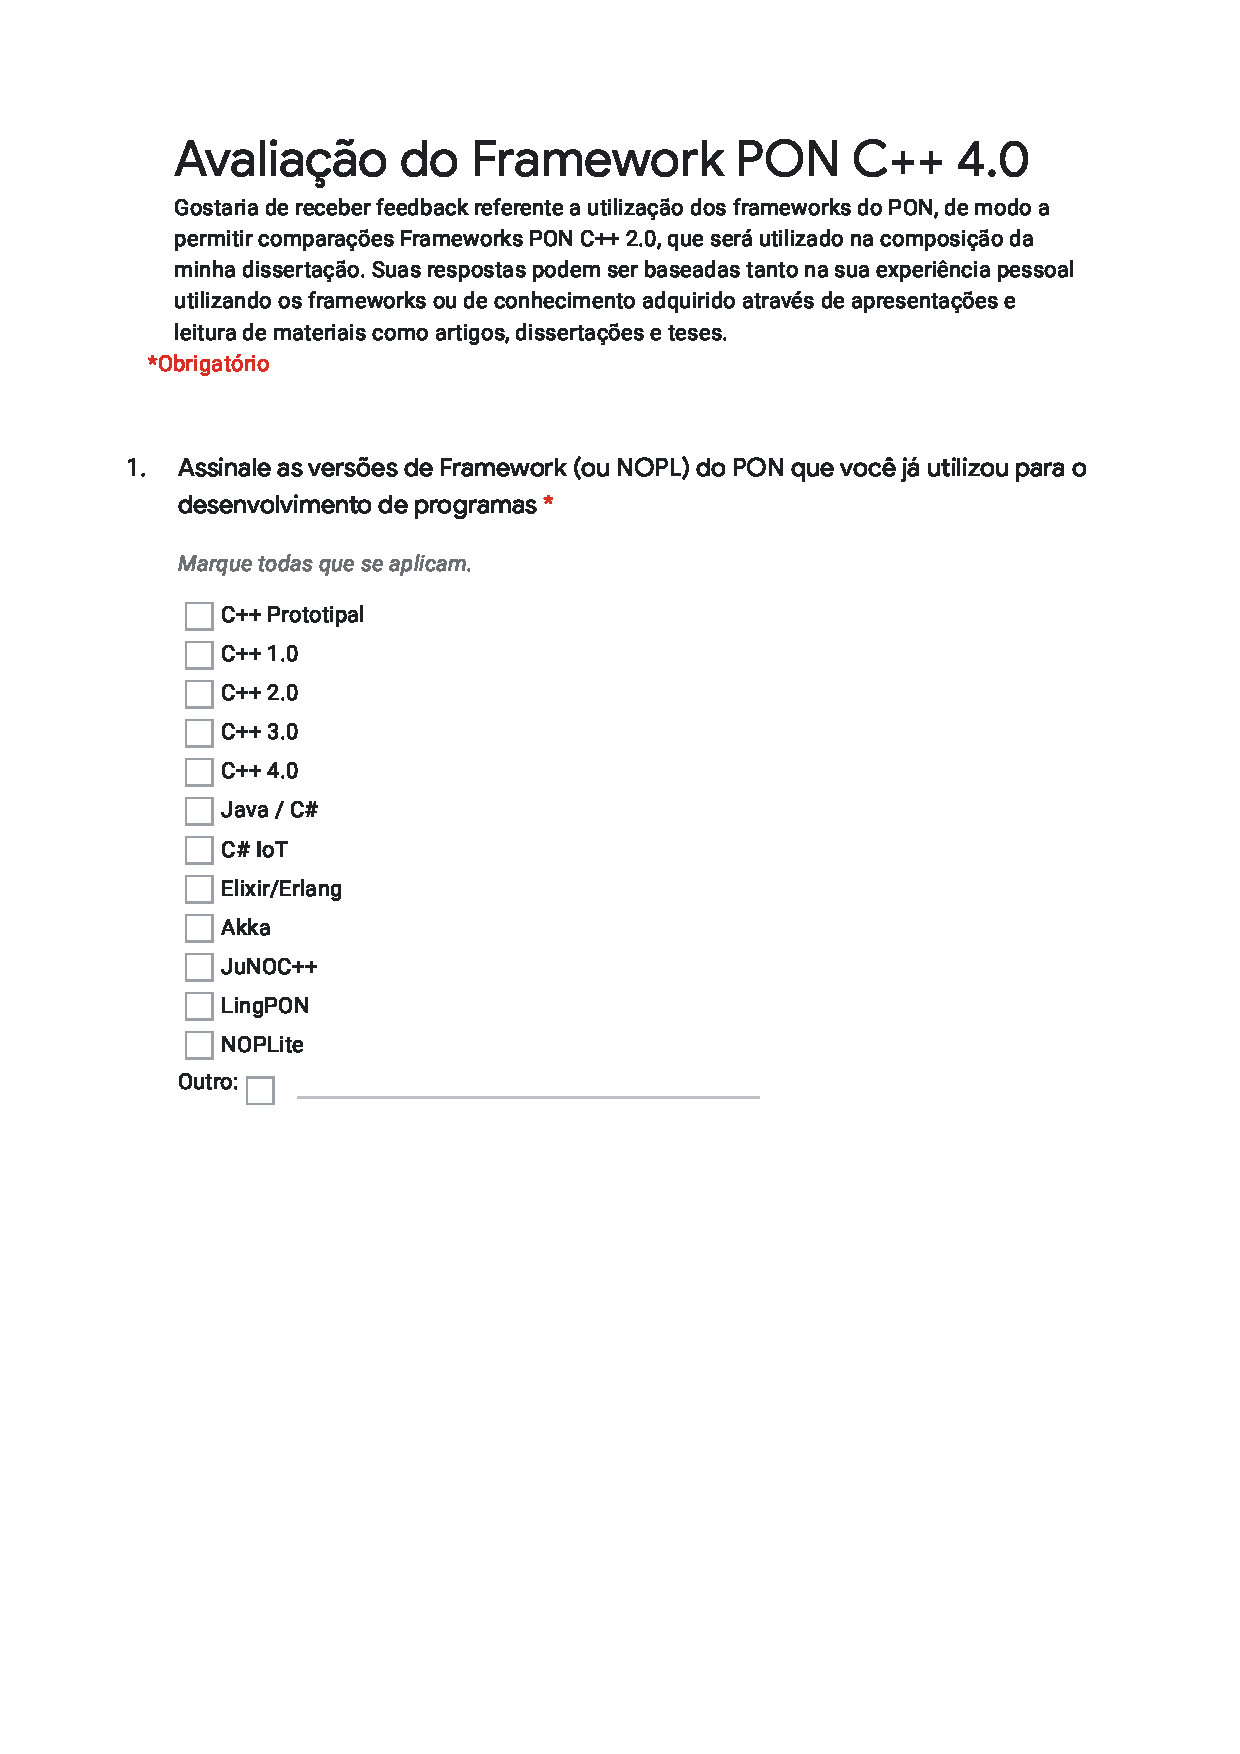
\includepdf[scale=0.8, pagecommand=\chapter*{Apêndice K}\label{ap:questionario}]{../extra/questionario.pdf}
\includepdf[scale=0.8, pages={2-5}]{../extra/questionario.pdf}
%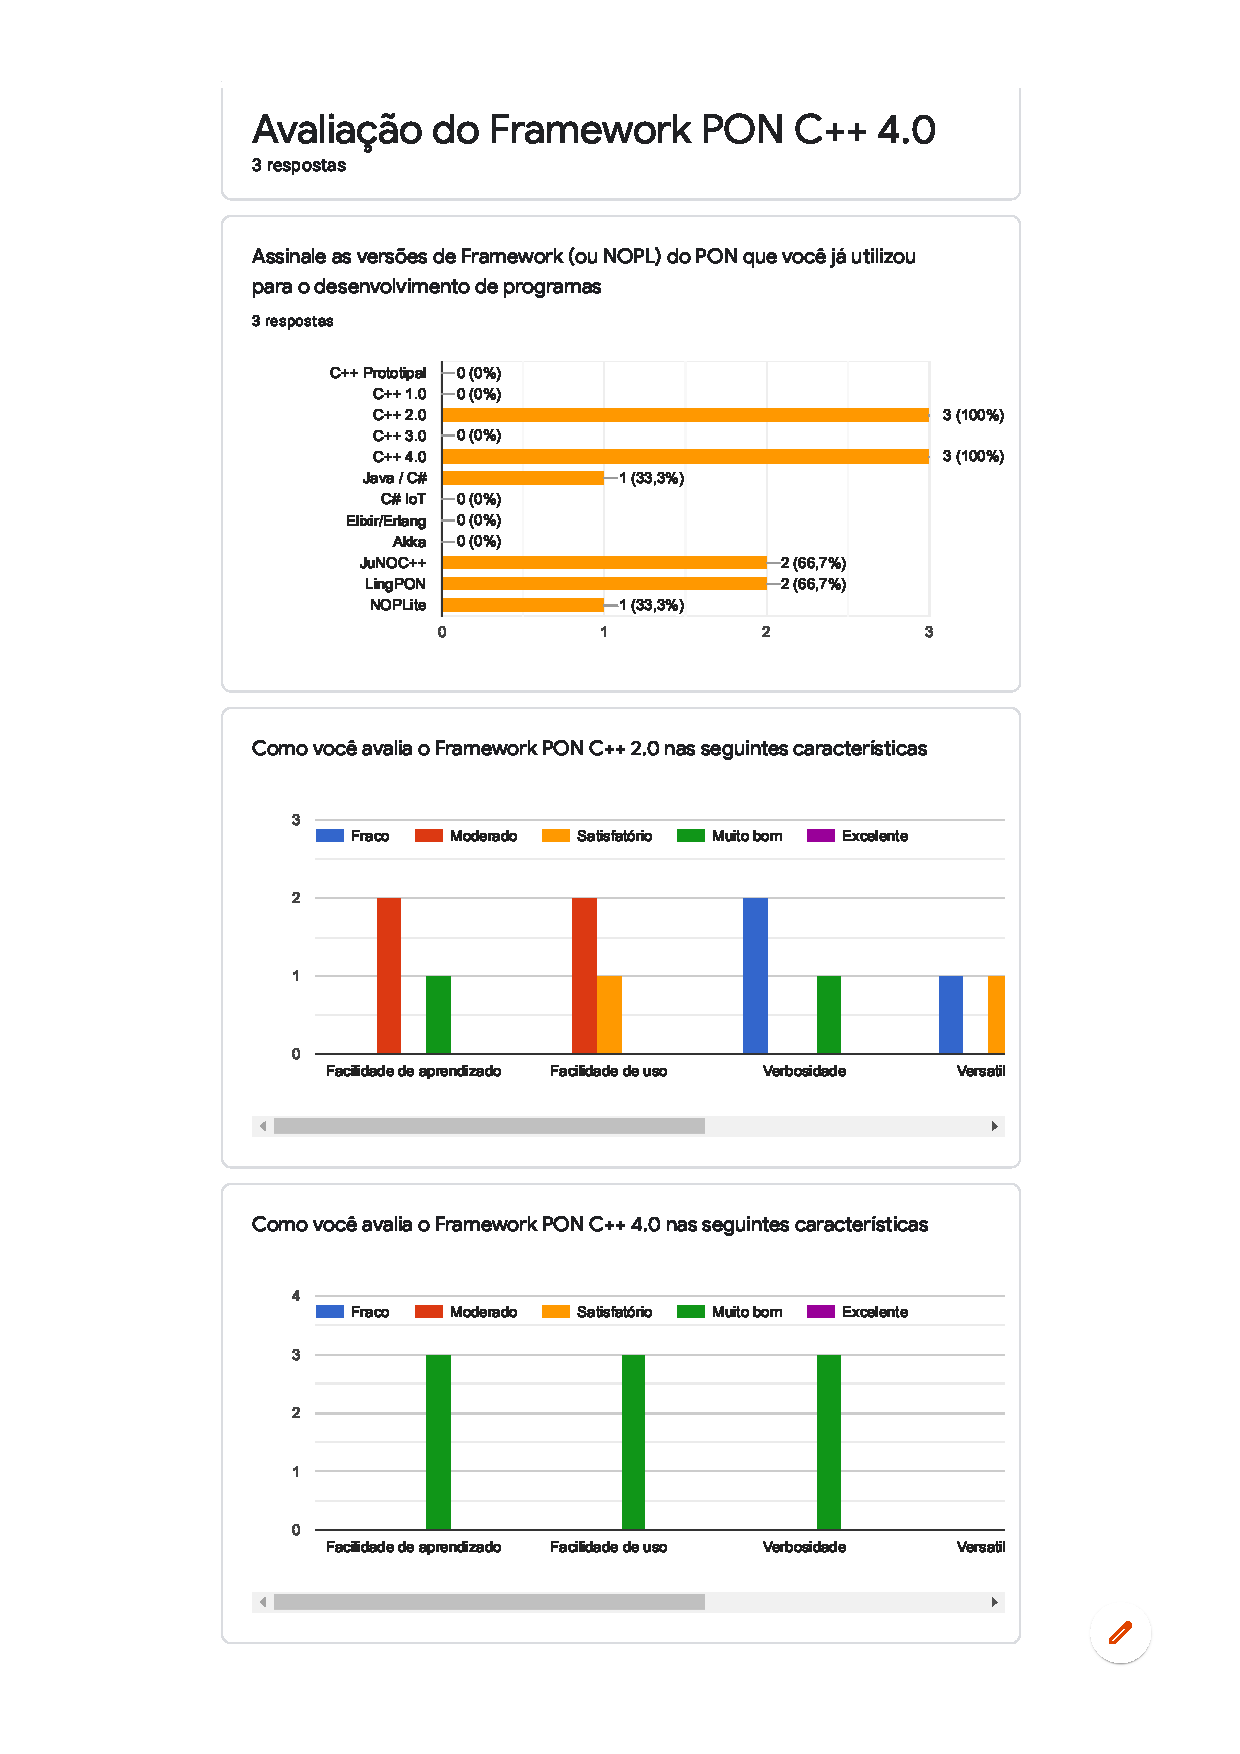
\includepdf[scale=0.8, pages={1-4}]{../extra/respostas_questionario.pdf}